\documentclass[tikz,border=4pt]{standalone}
\usepackage{pgfplots}
\usepgfplotslibrary{groupplots}
\pgfplotsset{compat=1.18}
\definecolor{proposedblue}{RGB}{46,94,170}
\definecolor{staticgray}{RGB}{128,136,148}
\definecolor{oraclegreen}{RGB}{69,145,98}
\definecolor{blackboxorange}{RGB}{218,132,55}
\definecolor{nomarginred}{RGB}{186,78,68}
\definecolor{vacationgold}{RGB}{204,151,55}
\definecolor{monepurple}{RGB}{126,93,159}
\definecolor{tealgreen}{RGB}{35,143,135}
\definecolor{deepviolet}{RGB}{98,80,154}
\begin{document}

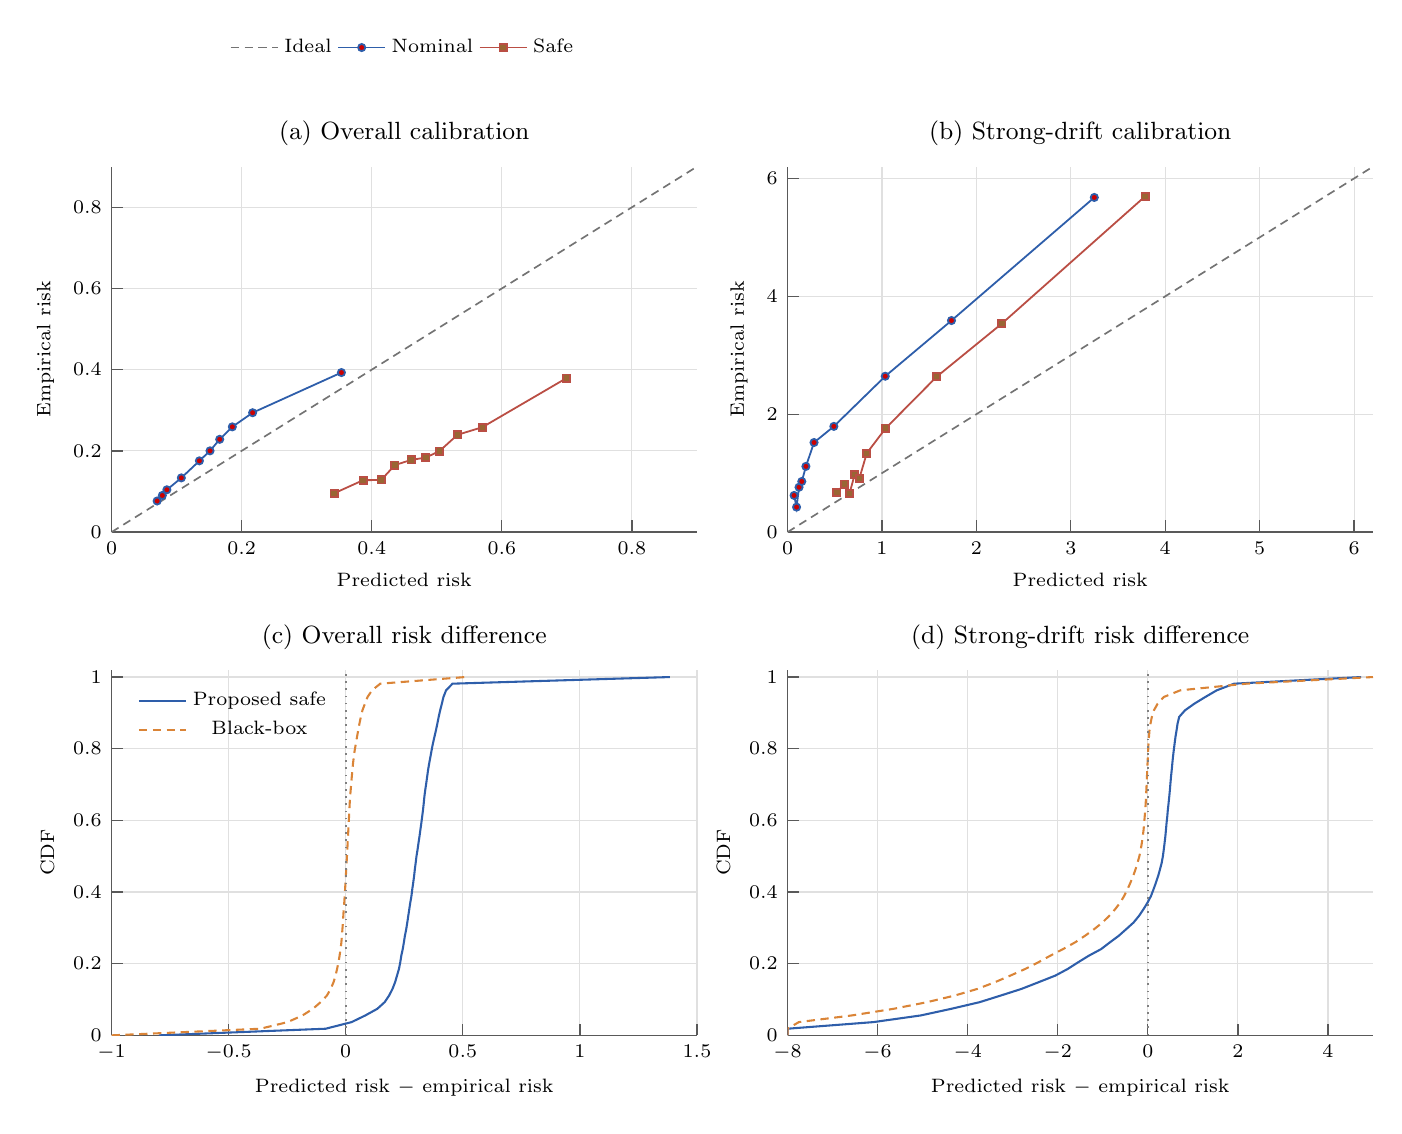
\begin{tikzpicture}
\begin{groupplot}[
    group style={group size=2 by 2, horizontal sep=1.15cm, vertical sep=1.75cm},
    width=3.55in,
    height=2.45in,
    ymajorgrids=true,
    xmajorgrids=true,
    grid style={black!12},
    axis x line*=bottom,
    axis y line*=left,
    axis line style={black!65, line width=0.45pt},
    tick style={black!65, line width=0.45pt},
    label style={font=\scriptsize},
    tick label style={font=\scriptsize},
    title style={font=\small, yshift=-0.5ex},
]
\nextgroupplot[
    title={(a) Overall calibration},
    xlabel={Predicted risk},
    ylabel={Empirical risk},
    xmin=0, xmax=0.90,
    ymin=0, ymax=0.90,
    legend style={at={(0.5,1.27)}, anchor=south, legend columns=3, draw=none, fill=none, font=\scriptsize},
]
\addplot+[black!55, densely dashed, line width=0.6pt, mark=none] coordinates {(0,0) (0.90,0.90)};
\addlegendentry{Ideal}
\addplot+[proposedblue, mark=*, mark size=1.3pt, line width=0.65pt] coordinates {
(0.0701,0.0766)
(0.0781,0.0902)
(0.0851,0.1042)
(0.1073,0.1335)
(0.1351,0.1755)
(0.1514,0.2001)
(0.1663,0.2285)
(0.1857,0.2592)
(0.2169,0.2940)
(0.3534,0.3929)
};
\addlegendentry{Nominal}
\addplot+[nomarginred, mark=square*, mark size=1.3pt, line width=0.65pt] coordinates {
(0.3422,0.0955)
(0.3867,0.1278)
(0.4145,0.1283)
(0.4356,0.1650)
(0.4604,0.1777)
(0.4833,0.1836)
(0.5043,0.1997)
(0.5318,0.2396)
(0.5701,0.2583)
(0.6993,0.3791)
};
\addlegendentry{Safe}

\nextgroupplot[
    title={(b) Strong-drift calibration},
    xlabel={Predicted risk},
    ylabel={Empirical risk},
    xmin=0, xmax=6.20,
    ymin=0, ymax=6.20,
]
\addplot+[black!55, densely dashed, line width=0.6pt, mark=none] coordinates {(0,0) (6.20,6.20)};
\addplot+[proposedblue, mark=*, mark size=1.3pt, line width=0.65pt] coordinates {
(0.0695,0.6218)
(0.0957,0.4238)
(0.1218,0.7611)
(0.1511,0.8588)
(0.1947,1.1146)
(0.2807,1.5198)
(0.4905,1.7934)
(1.0348,2.6442)
(1.7362,3.5892)
(3.2487,5.6772)
};
\addplot+[nomarginred, mark=square*, mark size=1.3pt, line width=0.65pt] coordinates {
(0.5225,0.6729)
(0.6027,0.8140)
(0.6570,0.6588)
(0.7104,0.9736)
(0.7608,0.9133)
(0.8392,1.3384)
(1.0403,1.7639)
(1.5804,2.6376)
(2.2692,3.5369)
(3.7857,5.6944)
};

\nextgroupplot[
    title={(c) Overall risk difference},
    xlabel={Predicted risk $-$ empirical risk},
    ylabel={CDF},
    xmin=-1.0, xmax=1.5,
    ymin=0, ymax=1.02,
    legend style={at={(0.03,0.97)}, anchor=north west, legend columns=1, draw=none, fill=none, font=\scriptsize},
]
\addplot+[proposedblue, line width=0.75pt, mark=none] coordinates {
(-0.7975,0.0000)
(-0.0856,0.0185)
(0.0252,0.0370)
(0.0838,0.0556)
(0.1350,0.0741)
(0.1662,0.0926)
(0.1853,0.1111)
(0.1997,0.1296)
(0.2108,0.1481)
(0.2190,0.1667)
(0.2273,0.1852)
(0.2329,0.2037)
(0.2373,0.2222)
(0.2435,0.2407)
(0.2483,0.2593)
(0.2527,0.2778)
(0.2584,0.2963)
(0.2629,0.3148)
(0.2671,0.3333)
(0.2714,0.3519)
(0.2757,0.3704)
(0.2807,0.3889)
(0.2841,0.4074)
(0.2882,0.4259)
(0.2920,0.4444)
(0.2951,0.4630)
(0.2987,0.4815)
(0.3022,0.5000)
(0.3068,0.5185)
(0.3108,0.5370)
(0.3151,0.5556)
(0.3190,0.5741)
(0.3229,0.5926)
(0.3266,0.6111)
(0.3302,0.6296)
(0.3332,0.6481)
(0.3360,0.6667)
(0.3397,0.6852)
(0.3439,0.7037)
(0.3478,0.7222)
(0.3517,0.7407)
(0.3565,0.7593)
(0.3618,0.7778)
(0.3669,0.7963)
(0.3725,0.8148)
(0.3789,0.8333)
(0.3855,0.8519)
(0.3914,0.8704)
(0.3970,0.8889)
(0.4034,0.9074)
(0.4106,0.9259)
(0.4174,0.9444)
(0.4286,0.9630)
(0.4560,0.9815)
(1.3845,1.0000)
};
\addlegendentry{Proposed safe}
\addplot+[blackboxorange, line width=0.75pt, mark=none, densely dashed] coordinates {
(-1.0000,0.0000)
(-0.3642,0.0185)
(-0.2482,0.0370)
(-0.1845,0.0556)
(-0.1400,0.0741)
(-0.1073,0.0926)
(-0.0803,0.1111)
(-0.0642,0.1296)
(-0.0521,0.1481)
(-0.0434,0.1667)
(-0.0370,0.1852)
(-0.0309,0.2037)
(-0.0262,0.2222)
(-0.0221,0.2407)
(-0.0185,0.2593)
(-0.0163,0.2778)
(-0.0141,0.2963)
(-0.0119,0.3148)
(-0.0103,0.3333)
(-0.0084,0.3519)
(-0.0062,0.3704)
(-0.0044,0.3889)
(-0.0026,0.4074)
(-0.0011,0.4259)
(0.0006,0.4444)
(0.0021,0.4630)
(0.0037,0.4815)
(0.0053,0.5000)
(0.0068,0.5185)
(0.0082,0.5370)
(0.0098,0.5556)
(0.0112,0.5741)
(0.0127,0.5926)
(0.0142,0.6111)
(0.0156,0.6296)
(0.0171,0.6481)
(0.0188,0.6667)
(0.0213,0.6852)
(0.0235,0.7037)
(0.0260,0.7222)
(0.0287,0.7407)
(0.0312,0.7593)
(0.0347,0.7778)
(0.0385,0.7963)
(0.0436,0.8148)
(0.0483,0.8333)
(0.0535,0.8519)
(0.0588,0.8704)
(0.0646,0.8889)
(0.0715,0.9074)
(0.0822,0.9259)
(0.0933,0.9444)
(0.1125,0.9630)
(0.1474,0.9815)
(0.5104,1.0000)
};
\addlegendentry{Black-box}
\addplot+[black!50, dotted, line width=0.6pt, mark=none, forget plot] coordinates {(0,0) (0,1.02)};

\nextgroupplot[
    title={(d) Strong-drift risk difference},
    xlabel={Predicted risk $-$ empirical risk},
    ylabel={CDF},
    xmin=-8.0, xmax=5.0,
    ymin=0, ymax=1.02,
]
\addplot+[proposedblue, line width=0.75pt, mark=none] coordinates {
(-8.0000,0.0000)
(-8.0000,0.0185)
(-6.0927,0.0370)
(-5.0406,0.0556)
(-4.3639,0.0741)
(-3.7354,0.0926)
(-3.2659,0.1111)
(-2.8060,0.1296)
(-2.4301,0.1481)
(-2.0551,0.1667)
(-1.7800,0.1852)
(-1.5501,0.2037)
(-1.3115,0.2222)
(-1.0375,0.2407)
(-0.8447,0.2593)
(-0.6459,0.2778)
(-0.4805,0.2963)
(-0.3174,0.3148)
(-0.1970,0.3333)
(-0.0967,0.3519)
(-0.0065,0.3704)
(0.0702,0.3889)
(0.1262,0.4074)
(0.1791,0.4259)
(0.2285,0.4444)
(0.2700,0.4630)
(0.3078,0.4815)
(0.3348,0.5000)
(0.3541,0.5185)
(0.3722,0.5370)
(0.3895,0.5556)
(0.4029,0.5741)
(0.4161,0.5926)
(0.4323,0.6111)
(0.4445,0.6296)
(0.4610,0.6481)
(0.4762,0.6667)
(0.4905,0.6852)
(0.5024,0.7037)
(0.5152,0.7222)
(0.5308,0.7407)
(0.5445,0.7593)
(0.5593,0.7778)
(0.5765,0.7963)
(0.5954,0.8148)
(0.6143,0.8333)
(0.6389,0.8519)
(0.6608,0.8704)
(0.6969,0.8889)
(0.8283,0.9074)
(1.0360,0.9259)
(1.2772,0.9444)
(1.5307,0.9630)
(1.9171,0.9815)
(4.7367,1.0000)
};
\addplot+[blackboxorange, line width=0.75pt, mark=none, densely dashed] coordinates {
(-8.0000,0.0000)
(-8.0000,0.0185)
(-7.7489,0.0370)
(-6.5715,0.0556)
(-5.6461,0.0741)
(-4.9031,0.0926)
(-4.2871,0.1111)
(-3.7857,0.1296)
(-3.3986,0.1481)
(-3.0538,0.1667)
(-2.7237,0.1852)
(-2.4345,0.2037)
(-2.1671,0.2222)
(-1.8831,0.2407)
(-1.6182,0.2593)
(-1.3957,0.2778)
(-1.1916,0.2963)
(-1.0079,0.3148)
(-0.8594,0.3333)
(-0.7263,0.3519)
(-0.6141,0.3704)
(-0.5261,0.3889)
(-0.4526,0.4074)
(-0.3868,0.4259)
(-0.3265,0.4444)
(-0.2740,0.4630)
(-0.2287,0.4815)
(-0.1875,0.5000)
(-0.1577,0.5185)
(-0.1327,0.5370)
(-0.1116,0.5556)
(-0.0941,0.5741)
(-0.0811,0.5926)
(-0.0690,0.6111)
(-0.0570,0.6296)
(-0.0468,0.6481)
(-0.0397,0.6667)
(-0.0328,0.6852)
(-0.0252,0.7037)
(-0.0189,0.7222)
(-0.0125,0.7407)
(-0.0062,0.7593)
(0.0010,0.7778)
(0.0081,0.7963)
(0.0155,0.8148)
(0.0252,0.8333)
(0.0376,0.8519)
(0.0599,0.8704)
(0.0896,0.8889)
(0.1372,0.9074)
(0.2185,0.9259)
(0.3559,0.9444)
(0.7205,0.9630)
(2.1862,0.9815)
(5.0000,1.0000)
};
\addplot+[black!50, dotted, line width=0.6pt, mark=none, forget plot] coordinates {(0,0) (0,1.02)};
\end{groupplot}
\end{tikzpicture}
\end{document}
